\section{Equational Reasoning}
\label{sec:equationalreasoning}

Verification is process of checking if the software does what the specification demands. To verify a program a specification is required. In the case of functions that implement an instance of the type classes of section \ref{sec:typeclasses} , the specification is defined in form of the type class laws.
This section will compare different verification techniques and describe the method equational reasoning by example. In \ref{sec:example} equational reasoning will be applied to proof the property of listing \ref{lst:applicative2monoid} in section \ref{sec:typeclasses}.

There are several ways to check the behavior of a program. 
We will describe the difference with a simple example. Given the following property:

\begin{equation}
  \label{eq:reverse_prop}
\text{reverse} (\text{reverse } xs) == xs  
\end{equation}

The equation \ref{eq:reverse_prop} expresses, if we apply \verb|reverse| two times on the same list \verb|xs| we get back the original list \verb|xs|. \verb|reverse| is the inverse of \verb|reverse|. Verification techniques allow us to check if equation \ref{eq:reverse_prop} holds. We describe 3 techniques:

\begin{description}
\item[Testing] Run the program with a selected input and check if it behaves as expected. In order to check the behavior a function evaluates both sites of the equation \ref{eq:reverse_prop} and compares the values.The following listing shows an example test.

\begin{verbatim}
input = [1,2,3]

test_reverse :: [Int] -> Bool
test_reverse xs = reverse (reverse xs) == xs
\end{verbatim}

The selected input is \verb|[1,2,3]|. \verb|test_reverse| evaluates to a Boolean expression to indicate if the property holds. It's necessary to run the program.
An advantage of this method is, that the programmer hasn't to define general properties. The specification is expressed with a concrete input value and a concrete output value. It's easier to think about a concrete input and the corresponding 
\item[Property-based testing] The input for the test program is generated randomly. The test are executed by a tool (e.g. Quickcheck)
\item[Proof] A Proof can shows that a property holds in all circumstances. To proof a property we use the technique equational reasoning. This technique requires knowledge of the function definition.
\end{description}

Figure \ref{fig:property_validation} compares the input coverage of the described methods. The rest of the section will only describe equational reasoning

\begin{figure}
  \centering
     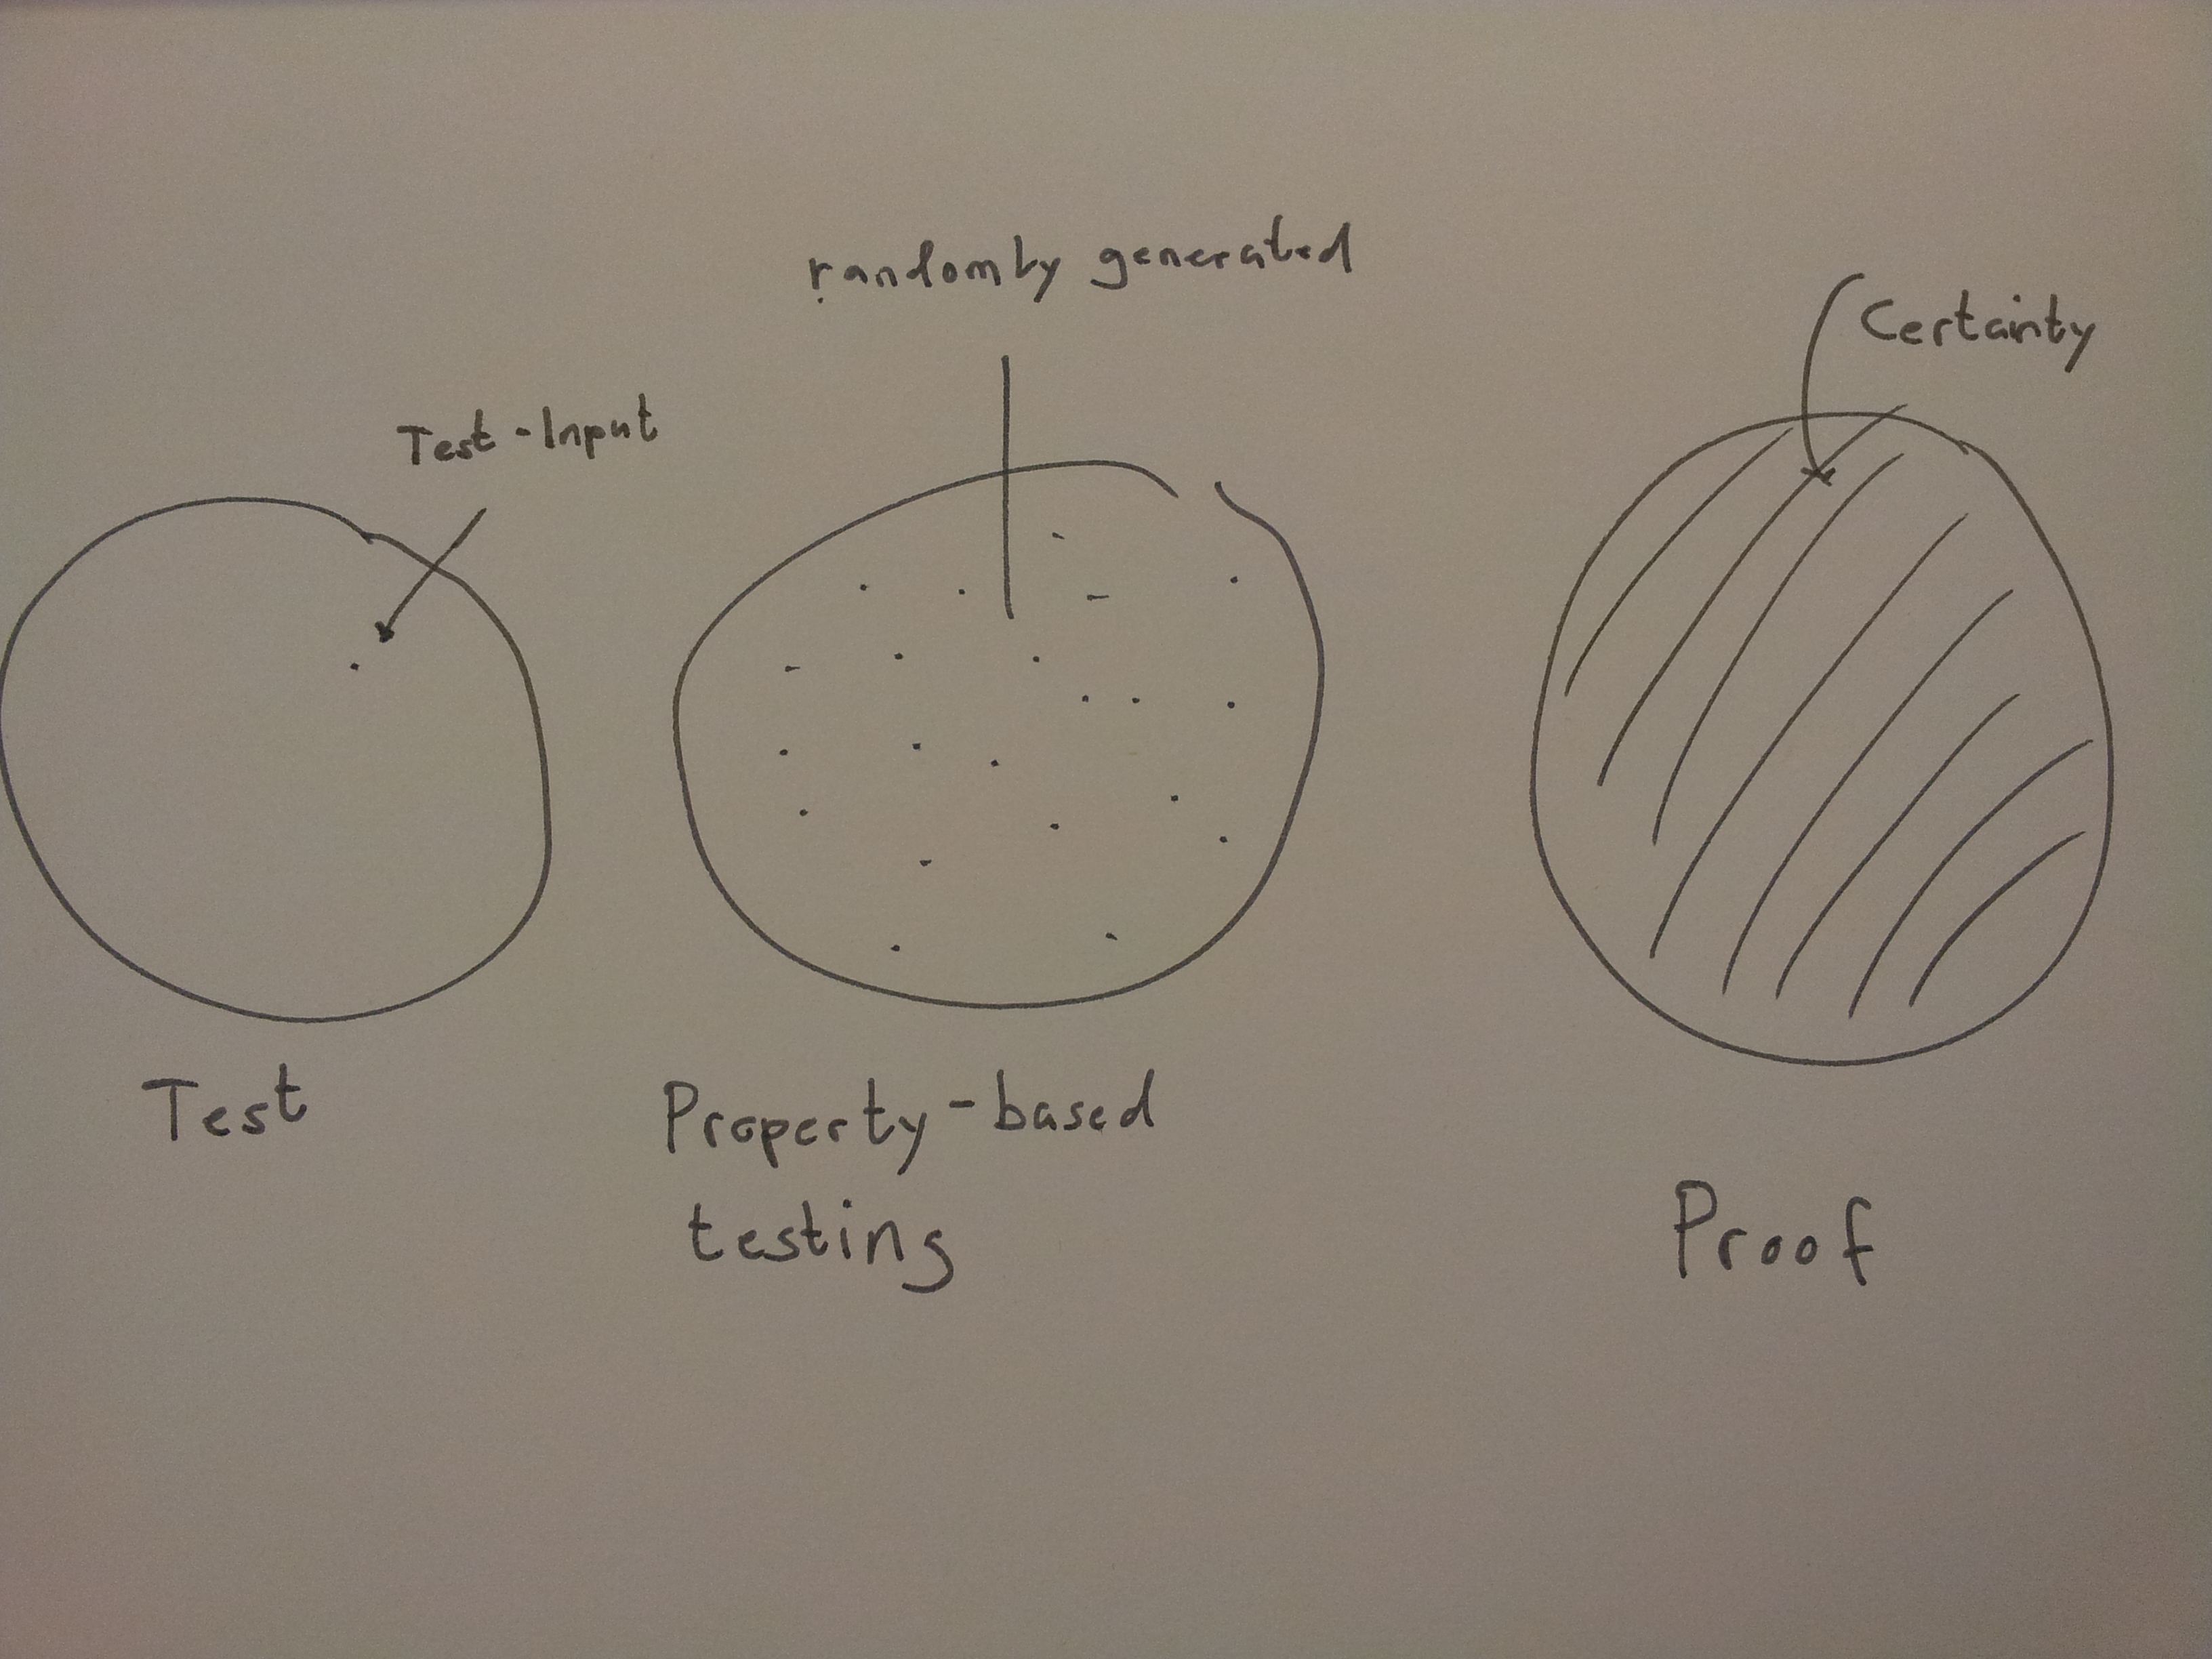
\includegraphics[width=0.9\textwidth]{comp}
  \caption{Comparison of test, property-based-testing and proof}
  \label{fig:property_validation}
\end{figure}

Equational reasoning isn't a method only used for or motivated from program verification. Equational reasoning is the process of substituting expressions. With equational reasoning we are able to show that certain algebraic properties hold.
For example, it's possible to show that

\begin{equation}
  \label{eq:sum}
  (x+a)(x+b) = x^2 + (a+b)x+ab
\end{equation}

is true. To show that the equality holds we have to substitute the expression on the left-hand side with the help of the basic algebraic properties of numbers (commutative, associative, distributive) \cite{hutton}. We could substitute the left-hand side as follows:

\begin{equation}
  \label{eq:algebra}
  (x+a)(x+b) = x^2 + ax + xb + ab \text{     (use distributivity)}
\end{equation}

\begin{equation}
x^2 + ax + bx + ab = x^2 + ax + bx + ab \text{     (use commutativity)}
\end{equation}

\begin{equation}
x^2 + ax + bx + ab = x^2 + (a + b)x + ab \text{     (use distributivity)}
\end{equation}

All we did, was substituting expression according the algebraic properties.

A function definition in Haskell means that we can substitute the left-hand side with the right-hand side and vice versa. This is possible because haskell is a pure functional language and side-effects are encapsulated in monads. Hence, we can use the same approach to proof that a property of Haskell program holds, as we used to reason about mathematical expressions. 
For example, it's possible to show that 
\begin{verbatim}
length [x] == 1
\end{verbatim}
no matter what \verb|x| is. If we have to prove this equality, we would first substitute \verb|length| with it's definition. If the definition is an expression with function calls we have to substitute them as well and so forth until only the value 1 remains.

This article will only describe proofs with programs, which halts. An evaluation can go on forever.
\begin{verbatim}
f x = 1 + f x
\end{verbatim}

The value of the expression is undefined. The proofs in this article hold only for defined expressions and finite lists..

Equational reasoning is use-full because
\begin{itemize}
\item it allows to verify properties of a program.
\item it can be used to eliminate expensive function call while preserving behavior
\end{itemize}

\subsection{Proof by structural induction}
\label{sec:induction}

If we apply simple substitution to a recursive function, we run into problems.
Consider the following definition:
\begin{verbatim}
length [] = 0
length (x:xs) = 1 + length xs
\end{verbatim}
If we substitute \verb|length x| with the definition \verb|1 + length xs|, we end up substituting \verb|length x| forever. A way to verify recursive programs is to use proof by structural induction.  
Structural induction for proofing a property can be used for list or algebraic data types with a recursive constructor (e.g. Tree).

 The principle of induction states, that it is sufficient to prove a property $p$ for the base case and that $p$ is preserved by the inductive case. In order to prove $p$, two steps are required:
 \begin{description}
 \item[Base case] Prove $p(0)$ is true.
 \item[Induction step] Prove $p(n+1)$ if $p(n)$ (induction hypothesis) is true.
 \end{description}

Proof by induction is similar to write a recursive function. Recursive functions use a base case (e.g. \verb|[]|, 0). 
If we use structural induction we proof the base case. We show that the property holds for a concrete input value (e.g. \verb|[]|, 0). 

In a recursive function definition we define \verb|f (x:xs)| and use \verb|f x| in the right-hand side. In the proof we show that $p(n+1)$ with the assumption $p(n)$.

We explain proof by structural induction with a simple example. Given the following property:
\begin{equation}
  \label{eq:lengthprop}
  \text{length (xs ++ ys)} = \text{(length xs) ++ (length ys)}
\end{equation}
We need the function definitions for \verb|length| and \verb|(++)|.
The Prelude functions \verb|length| and \verb|(++)| are defined as follows:
\begin{verbatim}
length [] = 0
length (x:xs) = 1 + length 
\end{verbatim}

\begin{verbatim}
[] ++ xs = xs
(x:xs) ++ ys = x:(xs++ys)
\end{verbatim}

\begin{description}
\item[Base case]
We have to show that property \ref{eq:lengthprop} holds for the base case. The base case, in this example, are the arguments \verb|[]| and a arbitrary list for \verb|ys|. It isn't necessary to replace \verb|ys| because, the definition of \verb|++| uses recursion over \verb|xs|. \verb|ys| will always be the same list.
In order to check if property \ref{eq:lengthprop} holds for the base case, we replace \verb|xs| with  \verb|[]|, leading to

\begin{verbatim}
length ([] ++ ys) = length [] + length ys
\end{verbatim}

We will evaluate the expression on the left-hand side and the right and side separately.
The left-hand side evaluates to

\begin{verbatim}
length ([] ++ ys) -- apply ++
length ys
\end{verbatim}

The right-hand side evaluates to 

\begin{verbatim}
length [] + length ys     -- apply length []
0 + length ys
length ys
\end{verbatim}

Both sides of the equation \ref{eq:lengthprop} are equal when evaluated with the the empty list \verb|[]| as argument. Hence, property \ref{eq:lengthprop} holds for base case.

\item[Induction step]
 We have to prove that
\begin{equation}
  \label{eq:induction}
    \text{length ((x:xs) ++ ys)} = \text{(length (x:xs)) ++ (length ys)}
\end{equation}

with the assumption (induction hypothesis)
\begin{equation}
  \label{eq:induction_hypothesis}
      \text{length (xs ++ ys)} = \text{(length xs) ++ (length ys)}
\end{equation}

Again, we evaluate the the left-hand side of equation \ref{eq:induction}.

\begin{program}
\begin{verbatim}
length ((x:xs) ++ ys)}     --apply definition of ++
length (x:(xs ++ ys))      --apply definition of length
1 + length (xs ++ ys)      --use induction hypothesis
1 + length xs + length ys
\end{verbatim}
\end{program}

If we evaluate the right-hand side of the induction step in equation  \ref{eq:induction} we get:
\begin{program}
\begin{verbatim}
length (x:xs) + length ys    -- apply definition of length
1 + length xs + length ys
\end{verbatim}
\end{program}

The last listing shows, that the equation \ref{eq:induction} follows from the induction hypothesis in equation \ref{eq:induction_hypothesis}. This completes the induction step and therefore the proof itself.
\end{description}

In order to apply equational reasoning we used definitions of all functions in your program. Hence, equational reasoning demands that we have access to the source code or that the the library, we are using already exhibits proved properties. If we use packages from hackage \footnote{http://hackage.haskell.org} Haskell we can browse the source code. 

Sometimes we can rely on proven properties. For example all types of the standard library, that are instance of a type class, satisfy the type class laws (see \ref{sec:typeclasses}) \cite{yorgey}. Some libraries exhibit properties in their documentation (e.g. pipes library of section \ref{sec:pipes} \cite{gonzales13})